\begin{figure}[H]
\centering
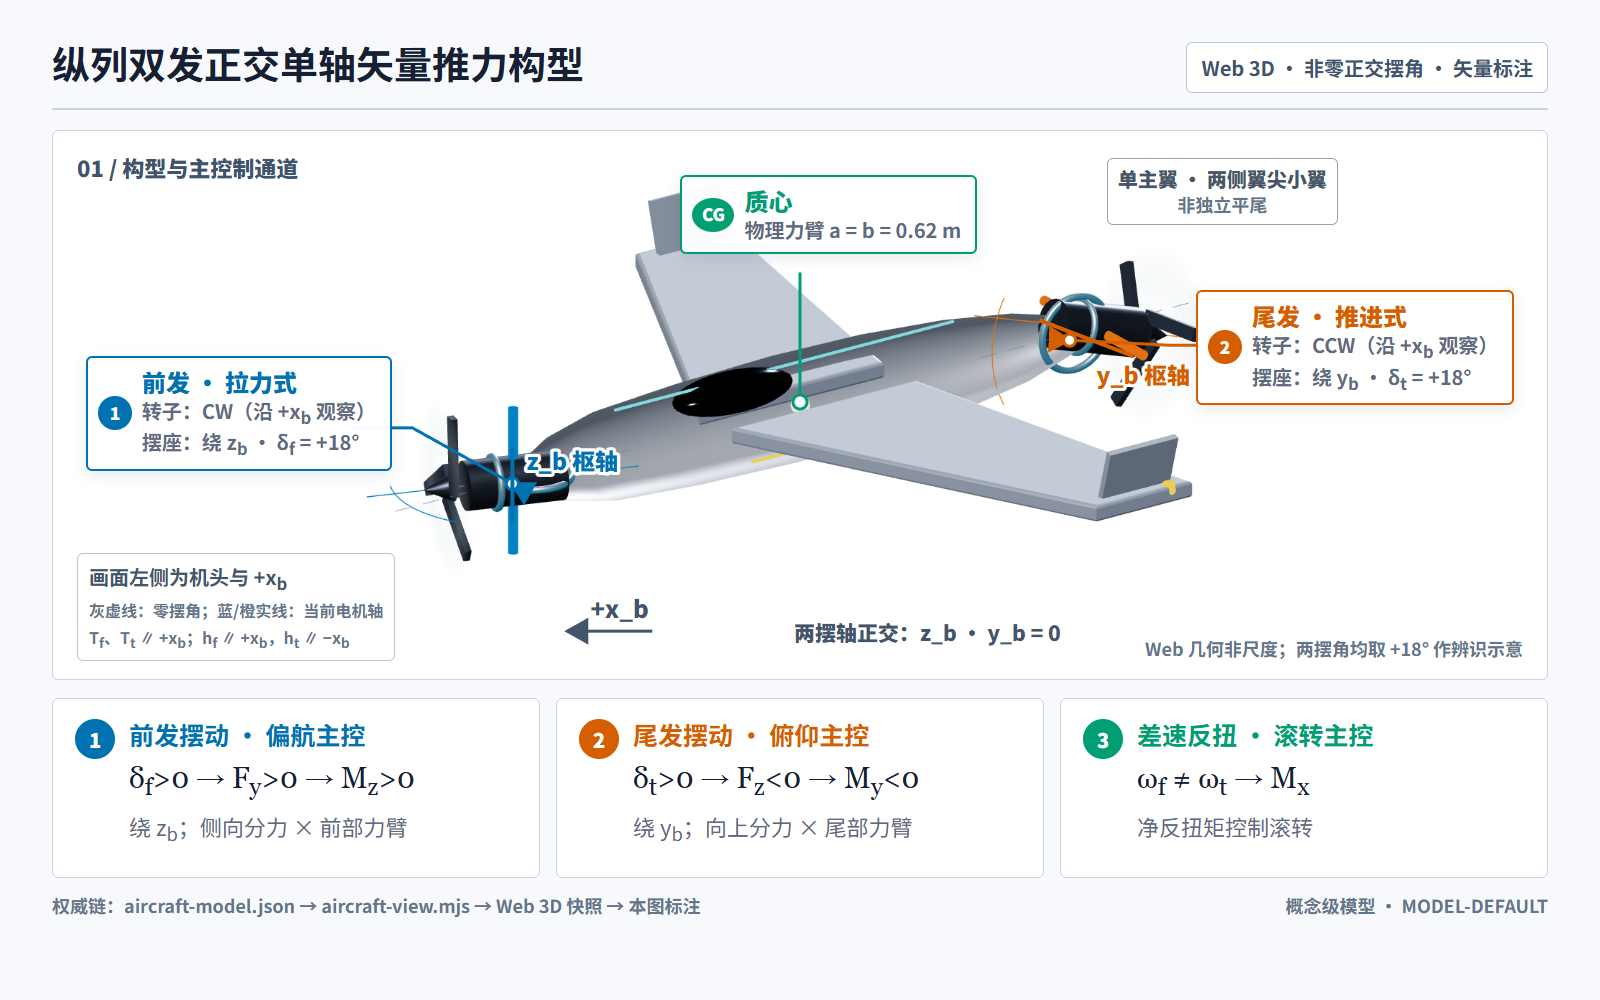
\includegraphics[width=0.99\linewidth]{fig/01-configuration.png}
\caption{纵列双发正交单轴矢量推力构型。底图直接复用Web程序化几何，并将前发固定为
$\delta_f=+18^\circ$绕$z_b$、尾发固定为$\delta_t=+18^\circ$绕$y_b$，以非零摆角直观区分两个正交单轴通道；
该姿态仅用于辨识，不代表同一配平或标定工作点。灰虚线表示零摆角$+x_b$基准，彩色实线表示当前电机轴，弧线表示各自运动平面内的摆角投影；
完整推力、旋向与角动量方向见图~\ref{fig:thrust_mapping}。渲染几何非尺度，物理力臂以\texttt{aircraft-model.json}中的
$a=b=0.62\,\mathrm{m}$为准。}
\label{fig:configuration}
\end{figure}
